\documentclass[12pt]{article}
\usepackage{graphicx}
\usepackage{amsmath, amssymb}
\usepackage{pgfplots}
\usepackage{lipsum}
\usepackage{geometry}
\geometry{margin=1in}
\usepackage{pgfplots}
\pgfplotsset{compat=1.18}
\usepackage{float}

\title{Tutoriat PS 1 - Random Variables}
\author{Mihai Duzi, Lucan Cristian, Lumînăraru Ionut}
\date{}

\begin{document}

\maketitle
\tableofcontents
\newpage

\section{Introduction}

\subsection{Types of random variables}

There are two types of random variables: \textbf{Discrete} and \textbf{Continuous}.  
Both are used to assign a value or weight to events — from winning or losing a bet to the occurrence of a natural event like a tornado.

\subsection{Terminology and Notation}

Let's start with an exercise.

I roll two dice at the same time. What is the probability that their sum is 8?

\[
\Omega = \{(i, j) \mid 1 \leq i \leq 6, 1 \leq j \leq 6\}
\]
\[
A = \{(i, j) \mid (i, j) \in \Omega, i + j = 8\}
\]
\[
P(A) = ?
\]

Let's define a function
\[
X(i, j) = i + j, \quad X: \Omega \rightarrow S, \text{ where } S = \{2, 3, \dots, 12\}
\]
Now,
\[
A = \{(i, j) \mid X(i,j) = 8\}
\]
We can write
\[
P(A) = P(X = 8) = \frac{5}{36}
\]

This function \( X \) is a \textbf{discrete random variable}.  
If \( S \) is at most countable, \( X \) is discrete; otherwise, \( X \) is continuous.

\section{Discrete Random Variables}

Beyond the already existing notation, we define the \textbf{probability mass function (pmf)}:
\[
p : S \rightarrow [0, 1]
\]
\[
p(x) = P(X = x)
\]
For our example above, \( p(8) = P(X = 8) = \frac{5}{36} \).  
The pmf uniquely identifies the distribution of the random variable.

For our example:
\[
X \sim 
\left(
\begin{array}{ccccccccccc}
2 & 3 & 4 & 5 & 6 & 7 & 8 & 9 & 10 & 11 & 12 \\[4pt]
\frac{1}{36} & \frac{2}{36} & \frac{3}{36} & \frac{4}{36} & \frac{5}{36} & \frac{6}{36} & \frac{5}{36} & \frac{4}{36} & \frac{3}{36} & \frac{2}{36} & \frac{1}{36}
\end{array}
\right)
\]

Now, what if I ask: what is the probability that the sum of the dice is smaller than 8?

\[
F(8) = P(X < 8) = \sum_{i=2}^{7} P(X = i)
\]

This defines the \textbf{cumulative distribution function (CDF)}, which gives the probability that \( X \) takes a value less than or equal to a given number.

\[
F(x) =
\left(
\begin{array}{ccccccccccc}
2 & 3 & 4 & 5 & 6 & 7 & 8 & 9 & 10 & 11 & 12 \\[4pt]
\frac{1}{36} & \frac{3}{36} & \frac{6}{36} & \frac{10}{36} & \frac{15}{36} & \frac{21}{36} & \frac{26}{36} & \frac{30}{36} & \frac{33}{36} & \frac{35}{36} & 1
\end{array}
\right)
\]

\subsection*{Visualizing the PMF and CDF}

\begin{center}
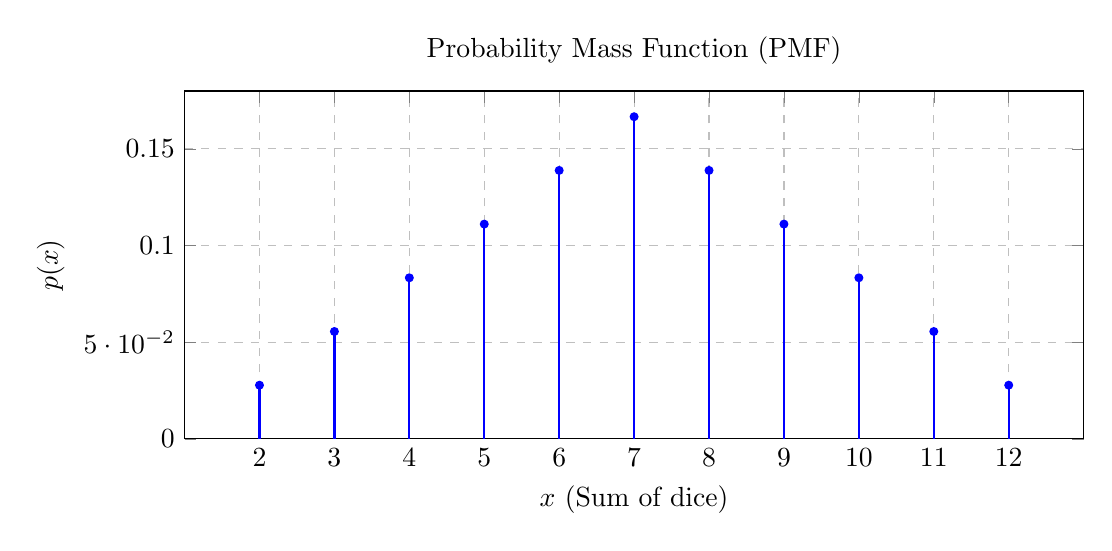
\begin{tikzpicture}
\begin{axis}[
    width=13cm, height=6cm,
    title={Probability Mass Function (PMF)},
    xlabel={$x$ (Sum of dice)},
    ylabel={$p(x)$},
    xtick={2,3,4,5,6,7,8,9,10,11,12},
    ytick={0,0.05,0.1,0.15,0.2},
    ymin=0, ymax=0.18,
    grid=major,
    ymajorgrids=true,
    xmajorgrids=true,
    grid style=dashed,
]
\addplot+[ycomb, thick, mark=*, mark options={scale=0.6}]
coordinates {
(2,1/36) (3,2/36) (4,3/36) (5,4/36) (6,5/36) (7,6/36) (8,5/36) (9,4/36) (10,3/36) (11,2/36) (12,1/36)
};
\end{axis}
\end{tikzpicture}

\vspace{1cm}

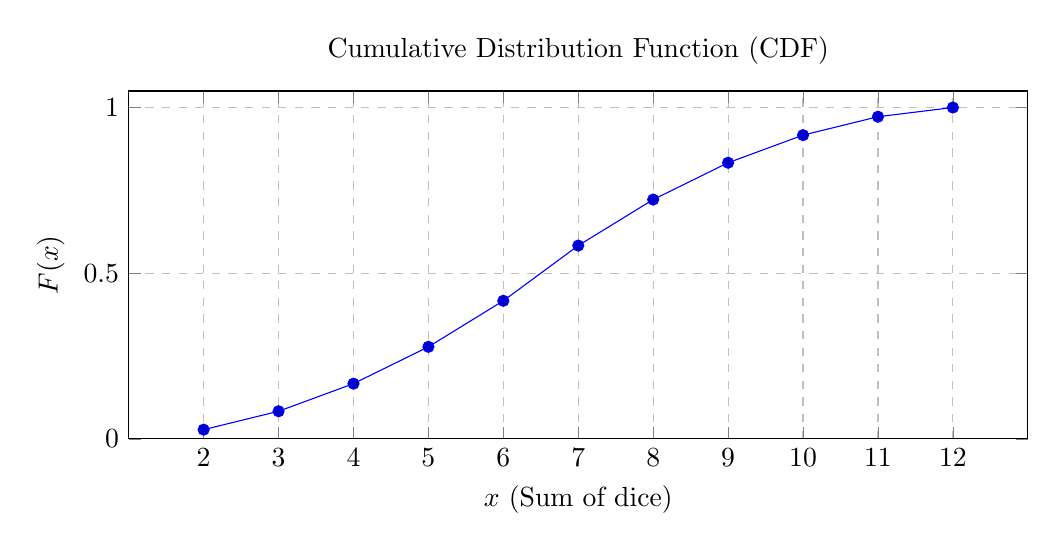
\begin{tikzpicture}
\begin{axis}[
    width=13cm, height=6cm,
    title={Cumulative Distribution Function (CDF)},
    xlabel={$x$ (Sum of dice)},
    ylabel={$F(x)$},
    xtick={2,3,4,5,6,7,8,9,10,11,12},
    ymin=0, ymax=1.05,
    grid=major,
    ymajorgrids=true,
    xmajorgrids=true,
    grid style=dashed,
]
\addplot+[mark=*] coordinates {
(2,1/36) (3,3/36) (4,6/36) (5,10/36) (6,15/36) (7,21/36) (8,26/36) (9,30/36) (10,33/36) (11,35/36) (12,1)
};
\end{axis}
\end{tikzpicture}
\end{center}

\subsection*{Observations}

We can now observe the following properties of the CDF:

1. \( F \) is \textbf{non-decreasing}. That is, the graph never goes down — symbolically, if \( a \leq b \), then \( F(a) \leq F(b) \).
2. \( 0 \leq F(a) \leq 1 \) for all real numbers \( a \).
3. \(\displaystyle \lim_{a \to -\infty} F(a) = 0\) and \(\displaystyle \lim_{a \to \infty} F(a) = 1.\)

\textbf{Random Variables Arithmetic}\newline
"+", "-", "$\times$" also work on random variables. \newline

The following random variable represents the distribution of points of a football match and their probabilities (3- Victory, 1 - Draw, 0 - Loss).\newline
\[
X \sim 
\left(
\begin{array}{ccc}
0 & 1 & 3 \\[4pt]
\frac{1}{4} & \frac{1}{4} & \frac{1}{2}
\end{array}
\right)
\]

Now what if we want the distribution of points of playing two football matches?
\(Y = X_1 + X_2 = 2 \times X\)

\textbf{Probability table:}

\[
\begin{array}{c|ccc}
X_1 \backslash X_2 & 0 & 1 & 3 \\ \hline
0 & 0 & 1 & 3 \\
1 & 1 & 2 & 4 \\
3 & 3 & 4 & 6
\end{array}
\]

Each combination occurs with probability equal to the product of the two individual probabilities:
\[
P(X_1=i, X_2=j) = P(X_1=i)\times P(X_2=j)
\]

\textbf{Resulting distribution:}

\[
Y = X_1 + X_2 \sim
\left(
\begin{array}{ccccccc}
0 & 1 & 2 & 3 & 4 & 6 \\[4pt]
\frac{1}{16} & \frac{1}{8} & \frac{1}{16} & \frac{1}{4} & \frac{1}{4} & \frac{1}{4}
\end{array}
\right)
\]

\subsection{Bernoulli Distribution}
\subsubsection{
    Definition
}
A Bernoulli distribution models binary events; the result is either \emph{failure} (0) or \emph{success} (1). It has a parameter \(p\) which represents the probability of success (and \(1-p\) is the probability of failure).

\subsubsection{
    Example
}
I throw a rigged coin that has probability \(\tfrac{1}{3}\) of being heads and \(\tfrac{2}{3}\) of being tails; I am trying to get heads.

This can be modeled as \(X \sim \mathrm{Bernoulli}\!\left(\tfrac{1}{3}\right)\). The pmf is
\[
P(X=x)=
\begin{cases}
\tfrac{1}{3}, & x=1,\\[4pt]
\tfrac{2}{3}, & x=0.
\end{cases}
\]
(Represented as a small table)
\[
X \sim
\left(
\begin{array}{cc}
1 & 0 \\[4pt]
\tfrac{1}{3} & \tfrac{2}{3}
\end{array}
\right)
\]

\subsubsection{
    Mean and Variance
}

\textbf{Mean: } E[X] = p\newline
\textbf{Variance:} Var[X] = p(1-p)\newline

Intuition: On average, if we make a lot of experiments, the probability of success will converge to p. 

\subsection{Binomial Distribution}
\subsubsection{
    Definition
}
This models multiple independent Bernoulli trials. It has two parameters: \(n\) — number of trials, and \(p\) — success probability per trial.

\subsubsection{
    Example
}
With the same (rigged) coin, what is the probability that I get 3 heads in 5 throws?

Let \(X\) be the number of heads in \(n=5\) independent throws. Each throw is Bernoulli\((p=\tfrac{1}{3})\).

\textbf{a) How many sequences of 5 throws contain 3 heads?}

The number of sequences of length \(n\) with exactly \(k\) heads is the binomial coefficient
\[
\binom{n}{k}=\frac{n!}{k!(n-k)!}.
\]
For this example (\(n=5,\;k=3\)):
\[
\binom{5}{3}=\frac{5!}{3!2!}=10.
\]

\textbf{(general)} Number of sequences with exactly \(k\) successes in \(n\) trials: \(\displaystyle \binom{n}{k}\).

\vspace{6pt}

\textbf{b) The actual problem: probability of exactly 3 heads in 5 throws}
\[
P(X=3)=\binom{5}{3}\left(\tfrac{1}{3}\right)^3\left(\tfrac{2}{3}\right)^2
=10\cdot\frac{1}{27}\cdot\frac{4}{9}=\frac{40}{243}\approx 0.1646.
\]

\textbf{Explanation: }\newline
$(\frac{1}{3})^3$ means we want 3 heads, $(\frac{2}{3})^2$ means we also want 2 tails. This results in exactly 3 heads.\newline

\textbf{Binomial distribution (general and current example).}

General:
\[
X\sim\mathrm{Binomial}(n,p),\qquad P(X=k)=\binom{n}{k}p^k(1-p)^{n-k},\quad k=0,1,\dots,n.
\]

Current example: \(X\sim\mathrm{Binomial}(5,\tfrac{1}{3})\). The PMF table is

\[
\begin{array}{c|cccccc}
k & 0 & 1 & 2 & 3 & 4 & 5\\\hline
\binom{5}{k} & 1 & 5 & 10 & 10 & 5 & 1\\[4pt]
P(X=k) & \tfrac{32}{243} & \tfrac{80}{243} & \tfrac{80}{243} & \tfrac{40}{243} & \tfrac{10}{243} & \tfrac{1}{243}
\end{array}
\]

\subsubsection{
    Right Tail Probability
}
\textbf{What is the probability that I get at least 3 heads in 5 throws?}
\[
P(X\ge3) = P(X = 3) + P(X = 4) + P(X = 5) = \frac{ \binom{5}{3}(1/3)^3(2/3)^2 + \binom{5}{4}(1/3)^4(2/3)^1 + \binom{5}{5}(1/3)^5 }{1}.
\]

Compute the numerators (common denominator \(243\)):
\[
P(X\ge3)=\frac{40+10+1}{243}=\frac{51}{243}=\frac{17}{81}\approx 0.2099.
\]

\textbf{(general)}:
\[
P(X\ge k_0)=\sum_{k=k_0}^{n}\binom{n}{k}p^k(1-p)^{n-k}.
\]

\subsubsection{
    Mean and Variance
}
For a Binomial distribution \(X \sim \mathrm{Binomial}(n, p)\):
\[
E[X] = n p, \qquad Var(X) = n p (1 - p)
\]

For our example (\(n = 5, p = \tfrac{1}{3}\)):
\[
E[X] = 5 \times \tfrac{1}{3} = \tfrac{5}{3} \approx 1.6667
\]
\[
Var(X) = 5 \times \tfrac{1}{3} \times \tfrac{2}{3} = \tfrac{10}{9} \approx 1.1111
\]
\[
\sigma_X = \sqrt{Var(X)} = \sqrt{\tfrac{10}{9}} \approx 1.054
\]

\textbf{Intuition for Mean and Variance:} Remember that Bin(n, p) is just n consecutive independent Bernoulli(p). That means Bin(n, p) = $ \sum_{i=1}^{n} Bernoulli(p) = n \times Bernoulli(p)$. Now $E[Bin(n, p)] = E[n \times Bernoulli(p)] = n \times E[Bernoulli(p)] = n \times p$.\newline
Variance is an exercise for you\newline

\subsubsection{
    Additivity Property
}

If \(X_1 \sim \mathrm{Binomial}(n_1, p)\) and \(X_2 \sim \mathrm{Binomial}(n_2, p)\) are \textbf{independent} random variables with the \textbf{same success probability} \(p\), then:
\[
X_1 + X_2 \sim \mathrm{Binomial}(n_1 + n_2, p).
\]

\textbf{Example:} Suppose you flip a coin with \(p=0.4\) success probability 10 times, then flip the same coin 15 more times. If \(X_1\) is the number of successes in the first 10 flips and \(X_2\) is the number in the next 15 flips, then:
\[
X_1 \sim \mathrm{Binomial}(10, 0.4), \quad X_2 \sim \mathrm{Binomial}(15, 0.4),
\]
and the total number of successes is:
\[
X_1 + X_2 \sim \mathrm{Binomial}(25, 0.4).
\]

\textbf{Note:} This property only holds when both binomial distributions have the \textbf{same} parameter \(p\). If the success probabilities differ, the sum is not binomial.


\subsection{Geometric Distribution}
\subsubsection{
    Definition
}
Geom(p) models the number of independent Bernoulli(p) probes until a success.

\subsubsection{
    Example
}
I throw the same coin from earlier and I stop when I get heads, what is the probability of having to throw it 5 times?

This means the first 4 throws were tails and the 5th was heads.\newline
\[
P(X = 5) = \left( \frac{2}{3} \right)^{4} \times \frac{1}{3}
\]

\textbf{Distribution representation from 1 to 5:}\newline
\[
\begin{array}{c|c}
x & P(X = x) \\ \hline
1 & \frac{1}{3} \\[4pt]
2 & \frac{2}{9} \\[4pt]
3 & \frac{4}{27} \\[4pt]
4 & \frac{8}{81} \\[4pt]
5 & \frac{16}{243}
\end{array}
\]

\textbf{General formula:}\newline
\[
P(X = k) = (1 - p)^{k - 1} \, p
\]

where \( p = \frac{1}{3} \) represents the probability of success (getting heads).\newline

\subsubsection{
    Left Tail Probability
}
\textbf{What is the probability of having to throw it less than 3 times?}\newline
\[
P(X < 3) = P(X=1) + P(X=2) = \frac{1}{3} + \frac{2}{9} = \frac{5}{9} \approx 0.5556
\]
\textbf{General:}
\[
P(X < k_0) = \sum_{i=1}^{k_0 - 1} (1-p)^{i-1} p = 1 - (1-p)^{k_0 - 1}
\]

\subsubsection{
    Mean and Variance
}
For a Geometric distribution \( X \sim \mathrm{Geom}(p) \):
\[
E[X] = \frac{1}{p}, \qquad Var(X) = \frac{1 - p}{p^2}.
\]

For our example (\( p = \tfrac{1}{3} \)):
\[
E[X] = \frac{1}{1/3} = 3
\]
\[
Var(X) = \frac{1 - 1/3}{(1/3)^2} = \frac{2/3}{1/9} = 6
\]
\[
\sigma_X = \sqrt{Var(X)} = \sqrt{6} \approx 2.449
\]

\textbf{Intuition for mean and variance:}\newline
On average, we expect to throw the coin \textbf{3 times} until we get heads, with moderate variability (\( \sigma_X \approx 2.45 \)) due to the chance of long sequences of tails.


\subsection{
    Hypergeometric Distribution
}

Let $Z$ be a random variable that gives the number of black balls that are drawn when a sample of $m$ balls is drawn (without replacement) from a lot of $n$ balls having $n_1$ black balls and $n_2$ white balls ($n_1 + n_2 = n$). 

The probability mass function of the random variable $Z$ is
\begin{equation}
p_Z(k) = \frac{\binom{n_1}{k} \binom{n-n_1}{m-k}}{\binom{n}{m}}, \quad k = 0, 1, \ldots, \min(n_1, m).
\end{equation}

We say that $Z$ has a hypergeometric distribution.


\subsection{
    Uniform Distribution
}

Uniform(n) creates a distribution where every number $v \in \{1, 2, ... n \}$ has the same probability, $\frac{1}{n}$. Simplest example is the distribution of a dice roll which can be modeled with Uniform(6).

\textbf{Mean:} E[X] = $\frac{n + 1}{2}$\newline
\textbf{Variance:} $\frac{n^2 - 1}{12}$

\subsection{
    Poisson Distribution
}

\subsubsection{Definition}

A random variable $X$ is \textbf{Poisson distributed} with parameter $\lambda > 0$, denoted $X \sim \text{Pois}(\lambda)$ or $X \sim P(\lambda)$, if:

$$X \in \{0, 1, 2, \ldots\} = \mathbb{N}$$

and its probability mass function is given by:

$$P(X = k) = e^{-\lambda} \frac{\lambda^k}{k!}, \quad k \in \mathbb{N}$$

\subsubsection{Interpretation and Usage}

The Poisson distribution models the \textbf{number of occurrences} of an event of interest in a context where:
\begin{itemize}
    \item The experiment is repeated a large number of times
    \item The probability of the event occurring is small
\end{itemize}

\textbf{Examples of applications:}
\begin{itemize}
    \item The number of customer arrivals at a counter within a specific time interval
    \item The number of spam emails received in one minute
    \item The number of system failures in a given period
    \item The number of phone calls received during a certain period
\end{itemize}

\subsubsection{Poisson Approximation of the Binomial Distribution}

The Poisson distribution arises as the \textbf{limit of the binomial distribution} under the following conditions:

Let $X_n \sim \text{Bin}(n, p_n)$ with $n \to \infty$, $p_n \to 0$ and $np_n \to \lambda > 0$.

Then:
$$\lim_{n \to \infty} P(X_n = k) = e^{-\lambda} \frac{\lambda^k}{k!}$$

\textbf{Proof of the Limit:}

Let $X_n \sim \text{Bin}(n, p_n)$ and let $\lambda = np_n$, which implies $p_n = \frac{\lambda}{n}$.
The binomial probability mass function is:
$$P(X_n = k) = \binom{n}{k} p_n^k (1 - p_n)^{n-k}$$

Substituting $p_n = \frac{\lambda}{n}$:
$$P(X_n = k) = \frac{n!}{k!(n-k)!} \left(\frac{\lambda}{n}\right)^k \left(1 - \frac{\lambda}{n}\right)^{n-k}$$

Rearranging the terms:
$$P(X_n = k) = \frac{n(n-1)\cdots(n-k+1)}{n^k} \cdot \frac{\lambda^k}{k!} \cdot \left(1 - \frac{\lambda}{n}\right)^n \cdot \left(1 - \frac{\lambda}{n}\right)^{-k}$$

We analyze the limit of each factor as $n \to \infty$:
\begin{enumerate}
    \item \textbf{Factor 1:} $\displaystyle \lim_{n \to \infty} \frac{n(n-1)\cdots(n-k+1)}{n^k} = \lim_{n \to \infty} \left(1 \cdot \left(1-\frac{1}{n}\right) \cdots \left(1-\frac{k-1}{n}\right)\right) = 1$
    \item \textbf{Factor 2:} $\displaystyle \lim_{n \to \infty} \frac{\lambda^k}{k!} = \frac{\lambda^k}{k!}$ (Does not depend on $n$)
    \item \textbf{Factor 3:} $\displaystyle \lim_{n \to \infty} \left(1 - \frac{\lambda}{n}\right)^n = e^{-\lambda}$ (Definition of the exponential limit)
    \item \textbf{Factor 4:} $\displaystyle \lim_{n \to \infty} \left(1 - \frac{\lambda}{n}\right)^{-k} = (1 - 0)^{-k} = 1$
\end{enumerate}

Multiplying the limits of the factors, we obtain:
$$\lim_{n \to \infty} P(X_n = k) = 1 \cdot \frac{\lambda^k}{k!} \cdot e^{-\lambda} \cdot 1 = e^{-\lambda} \frac{\lambda^k}{k!}$$

\textbf{Practical Rule:} The Poisson approximation is useful when:
\begin{itemize}
    \item $n$ is large (usually $n \geq 20$)
    \item $p$ is small (usually $p \leq 0.05$)
    \item The product $\lambda = np$ remains moderate (usually $\lambda \leq 10$)
\end{itemize}

In this case, we can approximate $\text{Bin}(n, p) \approx \text{Pois}(np)$.

\textbf{Example:} If $X \sim \text{Bin}(100, 0.02)$, then $X \approx \text{Pois}(2)$.

\subsubsection{Properties}

For $X \sim \text{Pois}(\lambda)$:
\begin{itemize}
    \item \textbf{Mean (Expected Value):} $E[X] = \lambda$
    \item \textbf{Variance:} $\text{Var}(X) = \lambda$
    \item \textbf{Moment Generating Function:} $M_X(t) = e^{\lambda(e^t - 1)}$
\end{itemize}

\textbf{Additivity Property:} If $X_1 \sim \text{Pois}(\lambda_1)$ and $X_2 \sim \text{Pois}(\lambda_2)$ are independent, then:
$$X_1 + X_2 \sim \text{Pois}(\lambda_1 + \lambda_2)$$
% ---------------------------------------------------------
\section{Expected Value and Variance}

% ---------------------------------------------------------
\subsection{Graphical interpretation of variance for a discrete random variable}

The variance measures how much the values of a discrete random variable differ from their mean.  
When the probabilities are concentrated around the mean, the variance is small.  
When the probabilities are spread farther from the mean, the variance becomes large.

\begin{figure}[H]
\centering
\begin{minipage}{0.48\textwidth}
\centering
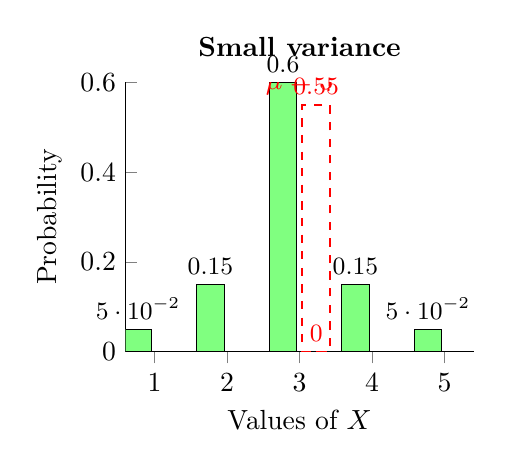
\begin{tikzpicture}
    \begin{axis}[
        ybar,
        ymin=0,
        ymax=0.6,
        ylabel={Probability},
        xlabel={Values of $X$},
        symbolic x coords={1,2,3,4,5},
        xtick=data,
        bar width=10pt,
        width=6cm,
        height=5cm,
        nodes near coords,
        every node near coord/.append style={font=\small},
        axis lines*=left,
        title={\textbf{Small variance}},
        ymajorgrids=false
    ]
    % Low variance distribution (centered)
    \addplot[fill=green!50] coordinates {
        (1,0.05)
        (2,0.15)
        (3,0.6)
        (4,0.15)
        (5,0.05)
    };
    % Mean line
    \addplot[dashed, red, thick] coordinates {(3,0) (3,0.55)};
    \node[above, red] at (axis cs:3,0.55) {$\mu=3$};
    \end{axis}
\end{tikzpicture}
\end{minipage}
\hfill
\begin{minipage}{0.48\textwidth}
\centering
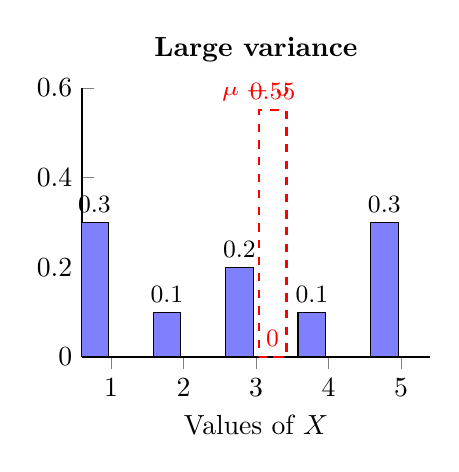
\begin{tikzpicture}
    \begin{axis}[
        ybar,
        ymin=0,
        ymax=0.6,
        xlabel={Values of $X$},
        symbolic x coords={1,2,3,4,5},
        xtick=data,
        bar width=10pt,
        width=6cm,
        height=5cm,
        nodes near coords,
        every node near coord/.append style={font=\small},
        axis lines*=left,
        title={\textbf{Large variance}},
        ymajorgrids=false
    ]
    % High variance distribution (spread out)
    \addplot[fill=blue!50] coordinates {
        (1,0.3)
        (2,0.1)
        (3,0.2)
        (4,0.1)
        (5,0.3)
    };
    % Mean line
    \addplot[dashed, red, thick] coordinates {(3,0) (3,0.55)};
    \node[above, red] at (axis cs:3,0.55) {$\mu=3$};
    \end{axis}
\end{tikzpicture}
\end{minipage}
\caption{Comparison between a discrete distribution with small variance (left) and large variance (right). 
When most probability mass is close to the mean, the variance is small; when it is spread far away, the variance increases.}
\end{figure}


\subsection{Visual illustration of variance using discrete points}

The concept of variance can also be visualized by representing data as individual points on a number line.  
When the points are close to the mean, the variance is small.  
When they are far from the mean, the variance is large.

\begin{figure}[H]
\centering
\begin{minipage}{0.48\textwidth}
\centering
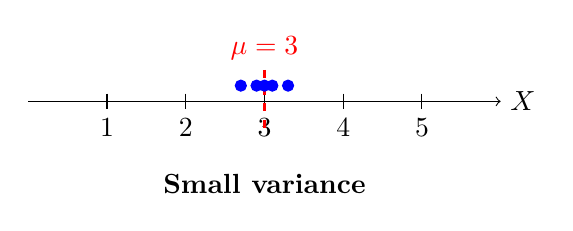
\begin{tikzpicture}
    % Number line
    \draw[->] (0,0) -- (6,0) node[right] {$X$};
    \foreach \x in {1,2,3,4,5} {
        \draw (\x,0.1) -- (\x,-0.1) node[below] {\x};
    }
    % Mean
    \draw[dashed, red, thick] (3,0.4) -- (3,-0.4);
    \node[above, red] at (3,0.4) {$\mu=3$};
    % Points (close to mean)
    \foreach \x in {2.7,2.9,3.0,3.1,3.3} {
        \filldraw[blue] (\x,0.2) circle (2pt);
    }
    \node[below,yshift=-0.3cm] at (3,-0.5) {\textbf{Small variance}};
\end{tikzpicture}
\end{minipage}
\hfill
\begin{minipage}{0.48\textwidth}
\centering
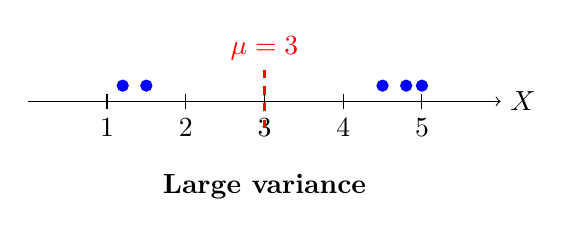
\begin{tikzpicture}
    % Number line
    \draw[->] (0,0) -- (6,0) node[right] {$X$};
    \foreach \x in {1,2,3,4,5} {
        \draw (\x,0.1) -- (\x,-0.1) node[below] {\x};
    }
    % Mean
    \draw[dashed, red, thick] (3,0.4) -- (3,-0.4);
    \node[above, red] at (3,0.4) {$\mu=3$};
    % Points (far from mean)
    \foreach \x in {1.2,1.5,4.5,4.8,5.0} {
        \filldraw[blue] (\x,0.2) circle (2pt);
    }
    \node[below,yshift=-0.3cm] at (3,-0.5) {\textbf{Large variance}};
\end{tikzpicture}
\end{minipage}
\caption{Illustration of variance using discrete points. 
When data points are close to the mean (left), variance is small. 
When they are far from the mean (right), variance is large.}
\end{figure}








\subsection{Properties of the Expectation}

If $c \in \mathbb{R}$ is a constant and $X$ and $Y$ are random variables defined on the same probability space $(\Omega, \mathcal{K}, P)$, then:
\[
E(c) = c, \qquad
E(cX) = cE(X), \qquad
E(X + Y) = E(X) + E(Y),
\]
\[
E(X) \le E(Y), \text{ if } X \le Y \text{ (i.e. } X(\omega) \le Y(\omega), \, \forall \omega \in \Omega).
\]


\subsection{Definitions and Moments}

\textbf{Definition 2.8.}  
Let $n \in \mathbb{N}$. The real number
\[
\beta_n := E(X^n) =
\begin{cases}
\displaystyle \sum_i x_i^n p_X(x_i), & \text{for discrete } X,\\[1em]
\displaystyle \int_{-\infty}^{\infty} x^n f_X(x)\,dx, & \text{for continuous } X.
\end{cases}
\]
If it exists, it is called the \textit{moment of order $n$} of $X$.

The \textit{central moment of order $n$} of $X$ is
\[
\mu_n = E\big[(X - m)^n\big] =
\begin{cases}
\displaystyle \sum_i (x_i - m)^n p_X(x_i), & \text{for discrete } X,\\[1em]
\displaystyle \int_{-\infty}^{\infty} (x - m)^n f_X(x)\,dx, & \text{for continuous } X.
\end{cases}
\]

\textbf{Definition 2.12.}  
Let $X$ be a random variable. The \textit{variance} (or \textit{dispersion}) of $X$ is the second central moment of $X$, denoted by $\sigma_X^2$, or simply $\sigma^2$, or $\mathrm{Var}(X)$.

Large values of $\sigma_X^2$ indicate a wide spread of the values of $X$ around the mean.  
Conversely, small values of $\sigma_X^2$ indicate a concentration of the values of $X$ near the mean.  
In the extreme case where $\sigma_X^2 = 0$, we have $X = m$ with probability 1 (i.e., the entire distribution mass is concentrated at the mean).

\textbf{Proposition.}  
The relationship between variance and the moments of $X$ is
\[
\sigma^2 = \beta_2 - m^2.
\]

\textbf{Proof.}
\[
\sigma^2 = E\big[(X - m)^2\big] = E[X^2 - 2mX + m^2]
= E[X^2] - 2mE[X] + m^2 = \beta_2 - m^2.
\]

\textbf{Other properties of the variance:}
\[
\mathrm{Var}(X) \ge 0, \qquad
\mathrm{Var}(c) = 0, \qquad
\mathrm{Var}(X + c) = \mathrm{Var}(X), \; \forall c \in \mathbb{R}, \qquad
\mathrm{Var}(cX) = c^2 \mathrm{Var}(X), \; \forall c \in \mathbb{R}.
\]

If $X$ is a random variable with mean $m$, its \textit{standard deviation} is defined as
\[
\sigma_X = \sqrt{E\big[(X - m)^2\big]}.
\]
An advantage of using $\sigma_X$ instead of $\sigma_X^2$ is that $\sigma_X$ has the same measurement unit as the mean, which allows direct comparison on the same scale and provides a measure of the degree of dispersion.

A dimensionless number (without measurement units) that characterizes the relative dispersion with respect to the mean and allows comparison between random variables measured in different units is the \textit{coefficient of variation}, defined as
\[
v_X = \frac{\sigma_X}{m_X}.
\]




\subsection{Logarithmic (series) distribution}
Consider the discrete distribution (also called the logarithmic or series distribution)
\[
P(X=k)=\frac{(1-p)^k}{-k\ln p},\qquad k=1,2,\dots,\qquad 0<p<1.
\]
The normalization uses the power series identity
\[
\sum_{k=1}^{\infty}\frac{(1-p)^k}{k}=-\ln p,
\]
so the pmf sums to 1.

\subsection{Expected value}

Compute
\[
E[X]=\sum_{k=1}^{\infty} k\,P(X=k)
      =\frac{1}{-\ln p}\sum_{k=1}^{\infty} k\frac{(1-p)^k}{k}
      =\frac{1}{-\ln p}\sum_{k=1}^{\infty}(1-p)^k.
\]
Let \(r=1-p\) (so \(0<r<1\)). Then
\[
\sum_{k=1}^{\infty} r^k=\frac{r}{1-r}=\frac{1-p}{p}.
\]
Hence
\[
\boxed{ \; E[X]=\frac{1-p}{-p\ln p} \; }.
\]

\subsection{Second moment and variance}

First,
\[
E[X^2]=\sum_{k=1}^{\infty} k^2 P(X=k)
      =\frac{1}{-\ln p}\sum_{k=1}^{\infty} k^2\frac{(1-p)^k}{k}
      =\frac{1}{-\ln p}\sum_{k=1}^{\infty} k(1-p)^k.
\]
Use the identity (valid for \(|r|<1\))
\[
\sum_{k=1}^{\infty} k r^k=\frac{r}{(1-r)^2}.
\]
With \(r=1-p\) this gives
\[
\sum_{k=1}^{\infty} k(1-p)^k=\frac{1-p}{p^2}.
\]
Therefore
\[
E[X^2]=\frac{1-p}{-p^2\ln p}.
\]
Thus the variance is
\[
\mathrm{Var}(X)=E[X^2]-\big(E[X]\big)^2
=\frac{1-p}{-p^2\ln p}-\left(\frac{1-p}{-p\ln p}\right)^{\!2}.
\]
A convenient algebraic simplification is
\[
\boxed{ \;
\mathrm{Var}(X)=\frac{(1-p)\big(-\ln p-(1-p)\big)}{p^2(-\ln p)^2}
\; }.
\]

\subsection{Worked exercise (numerical check)}

Take \(p=0.6\). Then \(1-p=0.4\) and \(-\ln p\approx 0.5108256\).

\[
E[X]=\frac{1-p}{-p\ln p}=\frac{0.4}{0.6\times 0.5108256}\approx 1.305.
\]

\[
\mathrm{Var}(X)=\frac{(1-p)\big(-\ln p-(1-p)\big)}{p^2(-\ln p)^2}
\approx \frac{0.4(0.5108256-0.4)}{0.36\times 0.5108256^2}\approx 0.472.
\]

These numerical values are useful to sanity-check an implementation or a simulation.


% ---------------------------------------------------------

\section{Continuous Random Variables}

For continuous random variables, the probability of taking any exact value is zero.  
Instead of a PMF, we use a \textbf{probability density function (pdf)} \( f(x) \) such that:
\[
P(a \leq X \leq b) = \int_{a}^{b} f(x) \, dx
\]
and
\[
\int_{-\infty}^{\infty} f(x) \, dx = 1.
\]

\end{document}
